\documentclass[11pt, a4paper, final]{article}

\usepackage[utf8]{inputenc}
\usepackage[T1]{fontenc}
\usepackage{textcomp}
\usepackage{babel}
\usepackage{amsmath, amssymb}

% Paquetes de configuracion
\input{./configuracion/paquetes}
\input{./configuracion/estilo}
\newcommand{\lad}{\hat{L}}
\newcommand{\lp}{\hat{L}_{+}}
\newcommand{\lm}{\hat{L}_{-}}
\newcommand{\lmi}{\hat{L}_{1-}}
\newcommand{\lmj}{\hat{L}_{2-}}
\newcommand{\lpj}{\hat{L}_{1-}}
\newcommand{\lpjj}{\hat{L}_{2-}}
\newcommand{\ls}{\hat{L}^{2}}
\newcommand{\eo}[1]{\Ket{#1}_1}
\newcommand{\et}[1]{\Ket{#1}_2}
\newcommand{\coef}[2]{\sqrt{#1\left( #1 + 1 \right) - #2\left( #2 - 1 \right)} \hbar }
\newcommand{\coefp}[2]{\sqrt{#1\left( #1 + 1 \right) - #2\left( #2 + 1 \right)} \hbar }

\input{./configuracion/bibliography_config}
\newcommand{\ttitle}{Main title}
\newcommand{\stitle}{\large{Subtitle}}
\newcommand{\finaldate}{\today}
\newcommand{\authorname}{José Antonio \textsc{Quiñonero Gris}}
\newcommand{\univname}{Universidad de Murcia}
\newcommand{\worktype}{Quick report}
\newcommand{\supname}{Supervisor Name \textsc{Surname}}
\newcommand{\degreename}{The degree}
\newcommand{\deptname}{Departamento de Química Física}
\newcommand{\facultyname}{Facultad de Química}
\newcommand{\institutename}{Institute name}
\newcommand{\centername}{Center name}
\newcommand{\kkeywords}{keyword1, keyword2}
\newcommand{\HRule}{\rule{.9\linewidth}{.6pt}} % New command to make the lines in the title page


% \usepackage{mathpazo}

\lstset{language=fortran,keywordstyle={\texttt}}
\NewDocumentCommand{\code}{v}{%
\texttt{#1}%
}

% \bibliography{./bibliografia/bibliografia_PE.bib}

\graphicspath{{./figuras/}}

\author{\authorname}
\title{
    \vspace{-2cm}
    \textbf{\ttitle}
}

\hypersetup{
pdfauthor={José Antonio Quiñonero Gris},
pdftitle={Worksheet 4.},
pdfsubject={Mathematical Foundation of Quantum Mechanics.},
pdfkeywords={Quantum Chemistry, Theoretical Chemistry, Computational Chemistry, Gaussian, Diels Alder}
}

% Fecha de creación: 14 de diciembre de 2022
% \date{}

\date{\today}

%
% --- INICIO DEL DOCUMENTO ---
%
\begin{document}
%
% --- Título ---
%
% \thispagestyle{empty}
% \maketitle
% \input{portada/portada}\afterpage{\blankpage}
% \afterpage{\blankpage}
% \input{portada/portada}\clearpage
\maketitle
%
% --- Texto ---
%
\graphicspath{{./figuras/}}
\textbf{Statement:} Calculate the Clebsh-Gordan coefficients corresponding to the composition of the
angular momenta $l_1 = 1$ and $l_2 = 2$ by using the step ladder angular momentum operators.\\ \vspace{1em}

\textbf{Solution:} Given the step ladder angular momentum operators
\begin{equation}\label{eq:ladder_operators}
    \lp = \lad_x + i \lad_y , \qquad \lm = \lad_x - i \lad_y,
\end{equation}

that act on the eigenfunctions of $\ls$, the spherical harmonics $\Ket{Y_{lm}} \equiv \Ket{l,m}$, as 
\begin{align}
    \lp \Ket{l, m} &= \sqrt{l\left( l + 1 \right) - m\left( m + 1 \right)} \hbar \Ket{l, m+1}, \label{eq:l_mas} \\
    \lm \Ket{l, m} &= \sqrt{l\left( l + 1 \right) - m\left( m - 1 \right)} \hbar \Ket{l, m-1}, \label{eq:l_menos}
\end{align}
and can be expressed, for each electron, as 
\begin{equation}\label{eq:separation_lad_op}
    \lp = \lpj + \lpjj ,
    \quad
    \lm = \lmi + \lmj.
\end{equation}
 
The possible values of the composition of the angular momenta $l$ and $m_l$ for the first electron, $\eo{l,m}$,
and for the second electron, $\et{l,m}$, are 
\begin{equation}
    l_1 = 2
    \begin{dcases}
        m_{l_1} = +2 & \, \eo{2,2}  \\
        m_{l_1} = +1 & \, \eo{2,1}  \\
        m_{l_1} = 0  & \, \eo{2,0}  \\
        m_{l_1} = -1 & \, \eo{2,-1} \\
        m_{l_1} = -2 & \, \eo{2,-2}
    \end{dcases}
    ; \quad 
    l_2 = 1
    \begin{dcases}
        m_{l_2} = +1 & \, \et{1,1}  \\
        m_{l_2} = 0  & \, \et{1,0}  \\
        m_{l_2} = -1 & \, \et{1,-1}
    \end{dcases}
    .
\end{equation}

Then, the total angular momentum $L = l_1 + l_2, \ldots, \left| l_1 - l_2 \right|$, is 
\begin{equation}
    L = 3,2,1.
\end{equation}

Now, for each component of the total angular momentum, the posible combinations of $\Ket{L,M}$ are
\begin{equation}
    L = 3
    \begin{dcases}
        M = +3 & \, \Ket{3,3}  \\
        M = +2 & \, \Ket{3,2}  \\
        M = +1 & \, \Ket{3,1}  \\
        M = 0  & \, \Ket{3,0}  \\
        M = -1 & \, \Ket{3,-1} \\
        M = -2 & \, \Ket{3,-2} \\
        M = -3 & \, \Ket{3,-3}
    \end{dcases}
    ; \quad 
    L = 2
    \begin{dcases}
        M = +2 & \, \Ket{2,2}  \\
        M = +1 & \, \Ket{2,1}  \\
        M = 0  & \, \Ket{2,0}  \\
        M = -1 & \, \Ket{2,-1} \\
        M = -2 & \, \Ket{2,-2}
    \end{dcases}
    ; \quad 
    L = 1
    \begin{dcases}
        M = +1 & \, \Ket{1,1}  \\
        M = 0  & \, \Ket{1,0}  \\
        M = -1 & \, \Ket{1,-1}
    \end{dcases}
    .
\end{equation}

The Clebsh-Gordan coefficients must be calculated for each of the combinations above.
%
%TODO: añadir mas explicacion sobre los coeficientes; que son, que representan y como calcularlos
%

% ------
% \section{$\boldsymbol{L = 3}$}
\section{$L = 3$}
% ------

Starting with the $L=3$, $M=3$ state, there is only one possible combination of states for electron 1 and electron 2, and that is 
\begin{equation}\label{eq:ket_3_3}
    \boxed{
        \Ket{3,3} = \eo{2,2} \et{1,1}.
    }
\end{equation}

(Note: the results are summarized at the end of the document)

In order to construct the rest of combinations for $L=3$, we can apply the lower operator $\lm$ [\cref{eq:l_menos}] to the
state $\Ket{3,3}$ to get $\Ket{3,2}$
\begin{equation}\label{eq:LHS_3_3}
    \lm \Ket{3,3} = \coef{3}{3} \Ket{3,2} = \sqrt{6} \hbar \Ket{3,2}. 
    \quad \left( = \text{LHS} \right)
\end{equation}

The ladder operator must be also applied to the right hand side (RHS) of the \cref{eq:ket_3_3}. Considering the separation of the
ladder operator as [\cref{eq:separation_lad_op}]:
\begin{equation}
    \lm = \lmi + \lmj,
\end{equation}
then 
\begin{equation}
    \lm \eo{2,2} \et{1,1} =
    \left( \lmi + \lmj \right) \eo{2,2} \et{1,1} =
    \lmi \eo{2,2} \et{1,1} + \lmj \eo{2,2} \et{1,1}
    ,
\end{equation}
and the fact that each component of the ladder operator acts only on the corresponding electron
\begin{align}
    \left( \lmi \eo{2,2} \right) \et{1,1} &= \left( \coef{2}{2} \eo{2,1} \right) \et{1,1} = 2 \hbar \eo{2,1} \et{1,1} , \\
    \left( \lmj \et{1,1} \right) \eo{2,2} &= \left( \coef{1}{1} \et{1,0} \right) \eo{2,2} = \sqrt{2} \hbar \eo{2,2} \et{1,0},
\end{align}
then 
\begin{equation}\label{eq:RHS_3_3}   
    \lm \eo{2,2} \et{1,1} = 2 \hbar \eo{2,1} \et{1,1} +  \sqrt{2} \hbar \eo{2,2} \et{1,0}.
     \quad \left( = \text{RHS} \right)
\end{equation}

Therefore, equating $\text{LHS} = \text{RHS}$ [equations \cref{eq:LHS_3_3} and \cref{eq:RHS_3_3}] 
\begin{equation}
    \sqrt{6} \hbar \Ket{3,2} 
    = 2 \hbar \eo{2,1} \et{1,1} +  \sqrt{2} \hbar \eo{2,2} \et{1,0},
\end{equation}
and factorizing $\sqrt{2} \hbar $ on the RHS
\begin{equation}
    \sqrt{6} \hbar \Ket{3,2} 
    = \sqrt{2} \hbar \left( \sqrt{2} \eo{2,1} \et{1,1} + \eo{2,2} \et{1,0} \right),
\end{equation}
then
\begin{equation}\label{eq:ket_3_2}
    \boxed{
        \Ket{3,2} = \frac{1}{\sqrt{3}} \left( \eo{2,2} \et{1,0} + \sqrt{2} \eo{2,1} \et{1,1} \right).
    }
\end{equation}

Just as before, the down operator $\lm$ can be applied again over $\Ket{3,2}$ to get $\Ket{3,1}$
\begin{equation}\label{eq:LHS_3_2}
    \lm \Ket{3,2} = \coef{3}{2} \Ket{3,1} = \sqrt{10} \hbar \Ket{3,1}. 
    \quad \left( = \text{LHS} \right)
\end{equation}
and to the RHS
\begin{equation}\label{eq:RHS_3_2_aux}
    \lm 
    \underbrace{ \left\{ \frac{1}{\sqrt{3}} \left( \sqrt{2} \eo{2,1} \et{1,1} + \eo{2,2} \et{1,0} \right) \right\} }_{\left\{\text{RHS}\right\}} =
    \sqrt{\frac{1}{3}} \left( \sqrt{2} \underbrace{\lm \eo{2,1} \et{1,1}}_{(*)} + \underbrace{\lm \eo{2,2} \et{1,0}}_{(**)} \right) .
\end{equation}

The result of the operations are calculated separately
\begin{align}
    \notag (*)  \ \lm \eo{2,1} \et{1,1} &= \left( \lmi \eo{2,1} \right) \et{1,1} + \left( \lmj \et{1,1} \right) \eo{2,1} =  \\
    \notag                              &= \coef{2}{1} \eo{2,0} \et{1,1} + \coef{1}{1} \et{1,0} \eo{2,1} = \\
                                        &= \sqrt{6} \hbar \eo{2,0} \et{1,1} + \sqrt{2} \hbar \et{1,0} \eo{2,1},
\end{align}
and
\begin{align}
    \notag (**) \, \lm \eo{2,2} \et{1,0} &= \left( \lmi \eo{2,2} \right) \et{1,0} + \left( \lmj \et{1,0} \right) \eo{2,2} =  \\
    \notag                              &= \coef{2}{2} \eo{2,1} \et{1,0} + \coef{1}{0} \et{1,-1} \eo{2,2} = \\
                                        &= 2 \hbar \eo{2,1} \et{1,0} + \sqrt{2} \hbar \et{1,-1} \eo{2,2}.
\end{align}

In \cref{eq:RHS_3_2_aux} 
\begin{equation}
    \begin{split}
        \lm \left\{ \text{RHS} \right\} &=
        \frac{ \hbar }{\sqrt{3}} \left\{ \sqrt{2} \left( \sqrt{6} \eo{2,0} \et{1,1} + \sqrt{2} \et{1,0} \eo{2,1} \right) + \right.\\
                                        & \left. \phantom{=} + 2 \eo{2,1} \et{1,0} + \sqrt{2} \hbar \et{1,-1} \eo{2,2} \right\}.
    \end{split}
\end{equation}

It can be rewritten as
\begin{align}
    \notag
    \lm \left\{ \text{RHS} \right\} &=
    \frac{ \hbar }{\sqrt{3}} \left( 2\sqrt{3} \eo{2,0} \et{1,1} + 2 \eo{2,1} \et{1,0} +
    2 \eo{2,1} \et{1,0} + \sqrt{2} \eo{2,2} \et{1,-1} \right) = \\
                                    &=
                                    \frac{ \hbar }{\sqrt{3}} \left( 2\sqrt{3} \eo{2,0} \et{1,1} + 4 \eo{2,1} \et{1,0} +
                                    \sqrt{2} \eo{2,2} \et{1,-1} \right).
\end{align}

Then, with \cref{eq:LHS_3_2} 
\begin{equation}
    \sqrt{10} \hbar \Ket{3,1} = 
    \frac{ \hbar }{\sqrt{3}} \left( 2\sqrt{3} \eo{2,0} \et{1,1} + 4 \eo{2,1} \et{1,0} +
                                    \sqrt{2} \eo{2,2} \et{1,-1} \right),
\end{equation}
therefore
\begin{equation}\label{eq:ket_3_1}
    \boxed{
        \Ket{3,1} = 
        \sqrt{\frac{1}{30}} \left( \sqrt{2} \eo{2,2} \et{1,-1} + 4 \eo{2,1} \et{1,0} + 2\sqrt{3} \eo{2,0} \et{1,1} \right).
    }
\end{equation}

Finally, applying again $\lm$ to $\Ket{3,1}$ to obtain $\Ket{3,0}$ 
\begin{equation}\label{eq:LHS_3_1}
    \lm \Ket{3,1} = \coef{3}{1} \Ket{3,0} = \sqrt{12} \hbar \Ket{3,0} = 2 \sqrt{3} \hbar \Ket{3,0}, \quad \left( =\text{LHS} \right)
\end{equation}
and to the RHS of the \cref{eq:ket_3_1}
\begin{equation}\label{eq:RHS_3_1}
    \lm \left\{ \text{RHS} \right\} =
    \sqrt{\frac{1}{30}} \left( 2 \sqrt{3} 
    \underbrace{\lm \eo{2,0} \et{1,1}}_{(*)}
    + 4 
    \underbrace{\lm \eo{2,1} \et{1,0} }_{(**)}
    + \sqrt{2} 
    \underbrace{\lm \eo{2,2} \et{1,-1} }_{(***)}
    \right)
\end{equation}

Calculating separately $\left( * \right)$
\begin{align}
    \notag (*) \ \lm \eo{2,0} \et{1,1} &= \lmi \eo{2,0} \et{1,1} + \lmj \et{1,1} \eo{2,0} = \\
    % \notag                             &= \coef{2}{0} \eo{2,-1} \et{1,1} + \\
    % \notag                             & \phantom{=} + \coef{1}{1} \et{1,0} \eo{2,0} = \\
                                       &= \sqrt{6} \hbar \eo{2,-1} \et{1,1} + \sqrt{2} \hbar \eo{2,0} \et{1,0},
\end{align}
and $\left( ** \right)$
\begin{align}
    \notag (**) \ \lm \eo{2,1} \et{1,0} &= \lmi \eo{2,1} \et{1,0} + \lmj \et{1,0} \eo{2,1} = \\
    % \notag                              &= \coef{2}{1} \eo{2,0} \et{1,0} +\\
    % \notag                              & \phantom{=} + \coef{1}{0} \et{1,-1} \eo{2,1} =\\
                                        &= \sqrt{6} \hbar \eo{2,0} \et{1,0} + \sqrt{2} \hbar \eo{2,1} \et{1,-1},
\end{align}
and, lastly, $\left( *** \right)$
\begin{align}
    \notag (***) \ \lm \eo{2,2} \et{1,-1} &= \lmi \eo{2,2} \et{1,-1} + \lmj \et{1,-1} \eo{2,2} = \\
    % \notag                                &= \coef{2}{2} \eo{2,1} \et{1,-1} + \\
    % \notag                                & \phantom{=} + \coef{1}{(-1)} \et{1,-2} \eo{2,2} = \\
                                          &= 2 \hbar \eo{2,1} \et{1,-1}.
\end{align}

Then, in \cref{eq:RHS_3_1} 
\begin{equation}
    \begin{split}
        \lm \left\{ \text{RHS} \right\} &=
        \sqrt{\frac{1}{30}} \left\{ 
            2 \sqrt{3} 
        \left( \sqrt{6} \hbar \eo{2,-1} \et{1,1} + \sqrt{2} \hbar \eo{2,0} \et{1,0} \right) + \right. \\
                                        & \phantom{=} + 4 \left( \sqrt{6} \hbar \eo{2,0} \et{1,0} + \sqrt{2} \hbar \eo{2,1} \et{1,-1} \right) + \\
                                        & \phantom{=} + \left. \sqrt{2} \left( 2 \hbar \eo{2,1} \et{1,-1} \right) \right\},
    \end{split}
\end{equation}
that, factorizing, can be rewritten as
\begin{equation}
    \lm \left\{ \text{RHS} \right\} =
    6 \hbar \sqrt{\frac{1}{15}} \left( 
    \eo{2,-1} \et{1,1} + \sqrt{3} \eo{2,0} \et{1,0} + \eo{2,1} \et{1,-1} \right).
\end{equation}

Doing $\text{LHS} = \text{RHS}$ with \cref{eq:LHS_3_1} 
\begin{equation}
    2 \sqrt{3} \hbar \Ket{3,0} =
    6 \hbar \sqrt{\frac{1}{15}} \left( 
    \eo{2,-1} \et{1,1} + \sqrt{3} \eo{2,0} \et{1,0} + \eo{2,1} \et{1,-1} \right),
\end{equation}
reads
\begin{equation}
    \boxed{
        \Ket{3,0} =
        \sqrt{\frac{1}{5}} \left( 
        \eo{2,1} \et{1,-1} + \sqrt{3} \eo{2,0} \et{1,0} + \eo{2,-1} \et{1,1} \right).
    }
\end{equation}

Now, the rest of combinations for $L=3$ can be calculated analogously starting with $\Ket{3,-3}$ and applying the rising ladder operator $\lp$ [\cref{eq:l_mas}].
The only combination for $\Ket{3,-3}$ is 
\begin{equation}
    \boxed{
        \Ket{3,-3} = \eo{2,-2} \et{1,-1}.
    }
\end{equation}

Applying $\lp$ to the LHS
\begin{equation}
    \lp \Ket{3,-3} = \coefp{3}{(-3)} \Ket{3,-2} = \sqrt{6} \hbar \Ket{3,-2}, \quad \left( = \text{LHS} \right)
\end{equation}
and to the RHS
\begin{equation}
    \lp \eo{2,-2} \et{1,-1} = \lpj \eo{2,-2} \et{1,-1} + \lpjj \et{1,-1} \eo{2,-2}.
\end{equation}

As
\begin{align}
    \lpj \eo{2,-2}  &= \coefp{2}{\left( -2 \right)} \eo{2,-1} = 2 \hbar \eo{2,-1}, \\
    \lpjj \et{1,-1} &= \coefp{1}{\left( -1 \right)} \et{1,0} = \sqrt{2} \hbar \et{1,0},
\end{align}
then
\begin{equation}
    \lp \eo{2,-2} \et{1,-1} = 2 \hbar \eo{2,-1} \et{1,-1} + \sqrt{2} \hbar \eo{2,-2} \et{1,0}.  \quad \left( =\text{RHS} \right)
\end{equation}

Equating LHS $=$ RHS 
\begin{equation}
    \begin{split}
        \sqrt{6} \hbar \Ket{3,-2} &=
        2 \hbar \eo{2,-1} \et{1,-1} + \sqrt{2} \hbar \eo{2,-2} \et{1,0} = \\
                                  &= \sqrt{2} \hbar \left( \sqrt{2} \eo{2,-1} \et{1,-1} + \eo{2,-2} \et{1,0} \right) ,
    \end{split}
\end{equation}
$\Ket{3,-2}$ is found and reads 
\begin{equation}
    \boxed{
        \Ket{3,-2} =
        \sqrt{\frac{1}{3}} \left( \sqrt{2} \eo{2,-1} \et{1,-1} + \eo{2,-2} \et{1,0} \right).
    }
\end{equation}
Now, $\lp$ can be applied again over $\Ket{3,-2}$
\begin{equation}
    \lp \Ket{3,-2} =
    \coefp{3}{\left( -2 \right)} \Ket{3,-1} =
    \sqrt{10} \hbar \Ket{3,-1}, \quad \left( =\text{LHS} \right)
\end{equation}
and for the RHS
\begin{equation}
    \lp 
    \left\{ \text{RHS} \right\}
    = 
    \sqrt{\frac{1}{3}} \left( \sqrt{2} \lp \eo{2,-1} \et{1,-1} + \lp \eo{2,-2} \et{1,0} \right),
\end{equation}
as
\begin{align}
    \notag \lp \eo{2,-1} \et{1,-1} &= \lpj \eo{2,-1} \et{1,-1} + \lpjj \et{1,-1} \eo{2,-1} = \\
    % \notag                         &= \coefp{2}{\left( -1 \right)} \eo{2,0} \et{1,-1} + \coefp{1}{\left( -1 \right)} \et{1,0} \eo{2,-1} = \\
    \notag                         &= \sqrt{6} \hbar \eo{2,0} \et{1,-1} + \sqrt{2} \hbar \et{1,0} \eo{2,-1} \\
                                   &= \sqrt{2} \hbar \left( \sqrt{3} \eo{2,0} \et{1,-1} + \eo{2,-1} \et{1,0} \right),
\end{align}
and
\begin{align}
    \notag \lp \eo{2,-2} \et{1,0}  &= \lpj \eo{2,-2} \et{1,0} + \lpjj \et{1,0} \eo{2,-2} = \\
    % \notag                         &= \coefp{2}{\left( -2 \right)} \eo{2,-1} \et{1,0} + \coefp{1}{0} \et{1,1} \eo{2,-2} = \\
    \notag                         &= 2 \hbar \eo{2,-1} \et{1,0} + \sqrt{2} \hbar \et{1,1} \eo{2,-2} \\
                                   &= \sqrt{2} \hbar \left( \sqrt{2} \eo{2,-1} \et{1,0} + \eo{2,-2} \et{1,1} \right),
\end{align}
then 
\begin{align}
    \notag \lp \left\{ \text{RHS} \right\} &= \sqrt{\frac{1}{3}} \left\{ \sqrt{2} 
        \sqrt{2} \hbar \left( \sqrt{3} \eo{2,0} \et{1,-1} + \eo{2,-1} \et{1,0} \right) \right. + \\
                                           & \left. \phantom{=} +
        \sqrt{2} \hbar \left( \sqrt{2} \eo{2,-1} \et{1,0} + \eo{2,-2} \et{1,1} \right)
        \right\} \\
                                           &= \sqrt{\frac{1}{3}} \hbar \left( 2 \sqrt{3} \eo{2,0} \et{1,-1} + 4 \eo{2,-1} \et{1,0} + \sqrt{2} \eo{2,-2} \et{1,1} \right).
                                           \quad \left( =\text{RHS} \right)
\end{align}
Doing LHS $=$ RHS
\begin{equation}
    \sqrt{10} \hbar \Ket{3,-1} =
    \sqrt{\frac{1}{3}} \hbar \left( 2 \sqrt{3} \eo{2,0} \et{1,-1} + 4 \eo{2,-1} \et{1,0} + \sqrt{2} \eo{2,-2} \et{1,1} \right),
\end{equation}
$\Ket{3,-1}$ reads
\begin{equation}
    \Ket{3,-1} =
    \sqrt{\frac{1}{30}} \left( 2 \sqrt{3} \eo{2,0} \et{1,-1} + 4 \eo{2,-1} \et{1,0} + \sqrt{2} \eo{2,-2} \et{1,1} \right),
\end{equation}
or
\begin{equation}
    \boxed{
        \Ket{3,-1} =
        \sqrt{\frac{1}{15}} \left( \sqrt{6} \eo{2,0} \et{1,-1} + 2\sqrt{2} \eo{2,-1} \et{1,0} + \eo{2,-2} \et{1,1} \right).
    }
\end{equation}

% ------
% \section{$\boldsymbol{L=2}$}
\section{$L=2$}
% ------

Now, the ladder operators can't be applied ver the already found combinations, since it is not the same value of $L$.
Therefore, the new states for $L=2$ are found imposing orthogonality conditions 
\begin{equation}\label{eq:orthogonality_condition}
    \Braket{L, M_L | L', M_{L'}} = 0 \qquad L' \not = L .
\end{equation}

Then, $\Ket{2,2}$ can be found imposing 
\begin{equation}\label{eq:orthog_cond_2_2}
    \Braket{3,2 | 2,2} = 0 .
\end{equation}
Rewriting $\Ket{3,2}$ from \cref{eq:ket_3_2} as 
\begin{equation}
    \Ket{3,2} = 
    \sqrt{\frac{1}{3}} \left( \sqrt{2} \eo{2,1} \et{1,1} + \eo{2,2} \et{1,0} \right) =
    \sqrt{\frac{1}{3}} \left( \sqrt{2} \Ket{\psi_1} + \Ket{\psi_2} \right),
\end{equation}
$\Ket{2,2}$ can be written as 
\begin{equation}\label{eq:lin_comb_2_2}
    \Ket{2,2} =
    c_1 \Ket{\psi_1} + c_2 \Ket{\psi_2}.
\end{equation}

Imposing now the orthogonality condition from \cref{eq:orthog_cond_2_2}
\begin{equation}
    \Braket{3,2 | 2,2} = 
    \sqrt{\frac{1}{3}} \left( \sqrt{2} \Bra{\psi_1} + \Bra{\psi_2} \right)
    \left( c_1 \Ket{\psi_1} + c_2 \Ket{\psi_2} \right)
    = 0,
\end{equation}
and operating considering that $\Braket{\psi_i | \psi_j} = \delta_{ij}$
\begin{align}
    \notag \Braket{3,2 | 2,2} &= 
    \sqrt{\frac{1}{3}} \left( 
          \sqrt{2} c_1 \Braket{\psi_1 | \psi_1}
                 + c_1 \Braket{\psi_2 | \psi_1}
        + \sqrt{2} c_2 \Braket{\psi_1 | \psi_2}
                 + c_2 \Braket{\psi_2 | \psi_2}
    \right) = \\
                              &= \sqrt{\frac{1}{3}} \left( \sqrt{2} c_1 + c_2 \right),
\end{align}
then 
\begin{equation}\label{eq:c1_-c2_2_2}
    \sqrt{\frac{1}{3}} \left( \sqrt{2} c_1 + c_2 \right) = 0 
    \implies
    c_1 = - \frac{1}{\sqrt{2}} c_2.
\end{equation}

Imposing now the normalisation condition 
\begin{equation}\label{eq:normalisation_condition}
    \sum_{i=1} \left| c_i \right|^2 = 1.
\end{equation}

Then 
\begin{equation}
    \left| c_1 \right|^2 + \left| c_2 \right|^2 = 1,
\end{equation}
substituting $c_1$ from \cref{eq:c1_-c2_2_2} 
\begin{equation}
    \left| - \frac{1}{\sqrt{2}} c_2 \right|^2 + \left| c_2 \right|^2 = \frac{3}{2} \left| c_2 \right|^2 = 1
    \implies 
    c_2 = \sqrt{\frac{2}{3}},
\end{equation}
and 
\begin{equation}
    c_1 = - \frac{1}{\sqrt{2}} c_2
        = - \frac{1}{\sqrt{2}} \sqrt{\frac{2}{3}}
        = - \frac{1}{\sqrt{3}}
\end{equation}

Then, \cref{eq:lin_comb_2_2} can be written as
\begin{equation}
    \Ket{2,2} =
    \frac{1}{\sqrt{3}} \left( - \Ket{\psi_1} + \sqrt{2} \Ket{\psi_2} \right) =
    \frac{1}{\sqrt{3}} \left( - \eo{2,1} \et{1,1} + \sqrt{2} \eo{2,2} \et{1,0} \right).
\end{equation}
Therefore, $\Ket{2,2}$ reads
\begin{equation}\label{eq:ket_2_2}
    \boxed{
    \Ket{2,2} =
    \sqrt{\frac{1}{3}} \left( \sqrt{2} \eo{2,2} \et{1,0} - \eo{2,1} \et{1,1} \right).
    }
\end{equation}

Now, the ladder operator can be applied to get the rest of combinations for $L=2$.
Applying $\lm$ over $\Ket{2,2}$ [\cref{eq:ket_2_2}]
\begin{equation}\label{eq:LHS_2_2}
    \lm \Ket{2,2} = 
    \coef{2}{2} \Ket{2,1} =
    2 \hbar \Ket{2,1}, 
    \quad \left( =\text{LHS} \right)
\end{equation}
and to the RHS 
\begin{equation}\label{eq:RHS_aux_2_1}
    \lm \left\{ \text{RHS} \right\} =
    \sqrt{\frac{1}{3}} \left( \sqrt{2} \lm \eo{2,2} \et{1,0} - \lm \eo{2,1} \et{1,1} \right).
\end{equation}
Calculating separately $\lm \eo{2,2} \et{1,0}$
\begin{align}
    \notag \lm \eo{2,2} \et{1,0} &= \lmi \eo{2,2} \et{1,0} + \lmj \et{1,0} \eo{2,2} = \\
    % \notag &= \coef{2}{2} \eo{2,1} \et{1,0} + \coef{1}{0} \et{1,-1} \eo{2,2} = \\
    \notag &= 2 \hbar \eo{2,1} \et{1,0} + \sqrt{2} \hbar \et{1,-1} \eo{2,2} = \\
           &= \sqrt{2} \hbar \left( \sqrt{2} \eo{2,1} \et{1,0} + \eo{2,2} \et{1,-1} \right),
\end{align}
and $\lm \eo{2,1} \et{1,1}$
\begin{align}
    \notag \lm \eo{2,1} \et{1,1} &= \lmi \eo{2,1} \et{1,1} + \lmj \et{1,1} \eo{2,1} = \\
    % \notag &= \coef{2}{1} \eo{2,0} \et{1,1} + \coef{1}{1} \et{1,0} \eo{2,1} = \\
    \notag &= \sqrt{6} \hbar \eo{2,0} \et{1,1} + \sqrt{2} \hbar \et{1,0} \eo{2,1} = \\
           &= \sqrt{2} \hbar \left( \sqrt{3} \eo{2,0} \et{1,1} + \eo{2,1} \et{1,0} \right),
\end{align}
then, on \cref{eq:RHS_aux_2_1}
\begin{align}\label{eq:RHS_2_2}
    \notag \lm \left\{ \text{RHS} \right\} &=
    \sqrt{\frac{1}{3}} \left\{ 
        \sqrt{2} \left[
            \sqrt{2} \hbar \left( \sqrt{2} \eo{2,1} \et{1,0} + \eo{2,2} \et{1,-1} \right)
        \right]
    \right. \\
    \notag & \phantom{=} - \left. 
        \sqrt{2} \hbar \left( \sqrt{3} \eo{2,0} \et{1,1} + \eo{2,1} \et{1,0} \right)
    \right\} = \\
    % \notag       &= 
    % \sqrt{\frac{2}{3}} \hbar \left\{ 
    %     \sqrt{2} \left( \sqrt{2} \eo{2,1} \et{1,0} + \eo{2,2} \et{1,-1} \right)
    %     -
    %     \left( \sqrt{3} \eo{2,0} \et{1,1} + \eo{2,1} \et{1,0} \right)
    % \right\} = \\
    % \notag       &= 
    % \sqrt{\frac{2}{3}} \hbar \left\{ 
    %     2 \eo{2,1} \et{1,0} + \sqrt{2} \eo{2,2} \et{1,-1}
    %     - \sqrt{3} \eo{2,0} \et{1,1} - \eo{2,1} \et{1,0}
    % \right\} = \\
    &= 
    \sqrt{\frac{2}{3}} \hbar \left\{ 
        \eo{2,1} \et{1,0} + \sqrt{2} \eo{2,2} \et{1,-1}
        - \sqrt{3} \eo{2,0} \et{1,1}
    \right\}.
    \quad \left( =\text{RHS} \right)
\end{align}

Equating LHS $=$ RHS with \cref{eq:LHS_2_2} and \cref{eq:RHS_2_2} 
\begin{equation}
    2 \hbar \Ket{2,1} =
    \sqrt{\frac{2}{3}} \hbar \left(
        \eo{2,1} \et{1,0} + \sqrt{2} \eo{2,2} \et{1,-1}
        - \sqrt{3} \eo{2,0} \et{1,1}
    \right),
\end{equation}
then
\begin{equation}
    \Ket{2,1} =
    \sqrt{\frac{1}{6}} \left(
        \eo{2,1} \et{1,0} + \sqrt{2} \eo{2,2} \et{1,-1}
        - \sqrt{3} \eo{2,0} \et{1,1}
    \right).
\end{equation}

Therefore, $\Ket{2,1}$ reads
\begin{equation}
    \boxed{
        \Ket{2,1} =
        \sqrt{\frac{1}{6}} \left(
            \sqrt{2} \eo{2,2} \et{1,-1}
            + \eo{2,1} \et{1,0}
            - \sqrt{3} \eo{2,0} \et{1,1}
        \right).
    }
\end{equation}

As before, applying $\lm$ over $\Ket{2,1}$ 
\begin{equation}\label{eq:LHS_2_1}
    \lm \Ket{2,1} =
    \coef{2}{1} \Ket{2,0} = 
    \sqrt{6} \hbar \Ket{2,0},
    \quad \left( =\text{LHS} \right)
\end{equation}
and to the RHS 
\begin{equation}\label{eq:RHS_2_1_aux}
    \lm \left\{ \text{RHS} \right\} =
        \sqrt{\frac{1}{6}} \left(
            \sqrt{2} \lm \eo{2,2} \et{1,-1}
            + \lm \eo{2,1} \et{1,0}
            - \sqrt{3} \lm \eo{2,0} \et{1,1}
        \right).
\end{equation}

Calculating separately $\lm \eo{2,2} \et{1,-1}$  
\begin{align}
    \notag
    \lm \eo{2,2} \et{1,-1} &=
    \lmi \eo{2,2} \et{1,-1} 
    + 
    \lmj \et{1,-1} \eo{2,2} = \\
    %
    %                        &=
    % \coef{2}{2} \eo{2,1} \et{1,-1}
    % +
    % \coef{1}{\left( -1 \right)} \et{1,-2} \eo{2,2} = \\
    %
                           &=
    2 \hbar \eo{2,1} \et{1,-1},
\end{align}
and $\lm \eo{2,1} \et{1,0}$
\begin{align}
    \notag
    \lm \eo{2,1} \et{1,0} &=
    \lmi \eo{2,1} \et{1,0} 
    + 
    \lmj \et{1,0} \eo{2,1} = \\
    %%
    % \notag
    %                        &=
    % \coef{2}{1} \eo{2,0} \et{1,0}
    % +
    % \coef{1}{0} \et{1,-1} \eo{2,1} = \\
    %%
    \notag
                           &=
    \sqrt{6} \hbar \eo{2,0} \et{1,0}
    +
    \sqrt{2} \hbar \et{1,-1} \eo{2,1} = \\
    %%
                           &=
    \sqrt{2} \hbar \left( 
        \sqrt{3} \eo{2,0} \et{1,0}
        +
        \eo{2,1} \et{1,-1} 
    \right),
\end{align}
and, lastly, $\lm \eo{2,0} \et{1,1}$
\begin{align}
    \notag
    \lm \eo{2,0} \et{1,1} &=
    \lmi \eo{2,0} \et{1,1} 
    + 
    \lmj \et{1,1} \eo{2,0} = \\
    %%
    % \notag
    %                        &=
    % \coef{2}{0} \eo{2,-1} \et{1,1}
    % +
    % \coef{1}{1} \et{1,0} \eo{2,0} = \\
    %%
    \notag
                           &=
    \sqrt{6} \hbar \eo{2,-1} \et{1,1}
    +
    \sqrt{2} \hbar \et{1,0} \eo{2,0} = \\
    %%
                           &=
    \sqrt{2} \hbar \left( 
        \sqrt{3} \eo{2,-1} \et{1,1}
        +
        \eo{2,0} \et{1,0}
    \right).
\end{align}

Then, in \cref{eq:RHS_2_1_aux}
\begin{align}\label{eq:RHS_2_1}
    \notag
    \lm \left\{ \text{RHS} \right\} &=
        \sqrt{\frac{1}{6}} \left\{
            \sqrt{2}
            \left( 2 \hbar \eo{2,1} \et{1,-1} \right)
            \right.
            \\
            %%
            \notag
            & \phantom{=} 
            +
            \sqrt{2} \hbar \left( 
                \sqrt{3} \eo{2,0} \et{1,0}
                +
                \eo{2,1} \et{1,-1} 
            \right)
            \\
            %%
            \notag
            & \phantom{=} 
            \left.
            - \sqrt{3}
            \left[
                \sqrt{2} \hbar \left( 
                    \sqrt{3} \eo{2,-1} \et{1,1}
                    +
                    \eo{2,0} \et{1,0}
                \right)
            \right]
        \right\}
        = \\
        %%
        % &=
        % \sqrt{\frac{1}{3}} \hbar \left\{
        %     2 \eo{2,1} \et{1,-1}
        %     +
        %     \sqrt{3} \eo{2,0} \et{1,0}
        %     +
        %     \eo{2,1} \et{1,-1} 
        %     -
        %     \sqrt{3} \left( 
        %         \sqrt{3} \eo{2,-1} \et{1,1}
        %         +
        %         \eo{2,0} \et{1,0}
        %     \right)
        % \right\}
        % = \\
        %%
        &=
        \sqrt{3} \hbar \left(
            \eo{2,1} \et{1,-1}
            -
            \eo{2,-1} \et{1,1}
        \right).
        \quad \left( =\text{RHS} \right)
\end{align}

Equating LHS $=$ RHS with \cref{eq:LHS_2_1} and \cref{eq:RHS_2_1} 
\begin{equation}
    \sqrt{6} \hbar \Ket{2,0} =
    \sqrt{3} \hbar \left(
            \eo{2,1} \et{1,-1}
            -
            \eo{2,-1} \et{1,1}
        \right).
\end{equation}

Then, $\Ket{2,0}$ reads 
\begin{equation}
    \boxed{
        \Ket{2,0} =
        \sqrt{\frac{1}{2}} \left(
            \eo{2,1} \et{1,-1}
            -
            \eo{2,-1} \et{1,1}
        \right).
    }
\end{equation}

Now, instead applying again $\lm$ to $\Ket{2,0}$, it is simpler to apply $\lp$ to $\Ket{2,-2}$.
Imposing the orthogonality condition [\cref{eq:orthogonality_condition}] between $\Ket{3,-2}$ and $\Ket{2,-2}$ 
\begin{equation}\label{eq:orthog_cond_2_-2}
    \Braket{3,-2 | 2,-2} = 0,
\end{equation}
rewriting $\Ket{3,-2}$ as 
\begin{equation}
    \Ket{3,-2} =
    \sqrt{\frac{1}{3}} \left( \sqrt{2} \eo{2,-1} \et{1,-1} + \eo{2,-2} \et{1,0} \right) =
    \sqrt{\frac{1}{3}} \left( \sqrt{2} \Ket{\psi_1} + \Ket{\psi_2} \right),
\end{equation}
and writing $\Ket{2,-2}$ as 
\begin{equation}\label{eq:aux_2_-2}
    \Ket{2,-2} =
    c_1 \Ket{\psi_1} + c_2 \Ket{\psi_2}.
\end{equation}

In \cref{eq:orthog_cond_2_-2}
\begin{align}
    \notag
    \Braket{3,-2 | 2,-2} &=
    \sqrt{\frac{1}{3}} \left[  
        \left( \sqrt{2} \Bra{\psi_1} + \Bra{\psi_2} \right)
        \left( c_1 \Ket{\psi_1} + c_2 \Ket{\psi_2} \right)
    \right]
    = \\
    %%
    \notag
    &=
    \sqrt{\frac{1}{3}} \left[  
        \sqrt{2} c_1 \Braket{\psi_1 | \psi_1} +
        \sqrt{2} c_2 \Braket{\psi_1 | \psi_2} +
        c_1 \Braket{\psi_2 | \psi_1} +
        c_2 \Braket{\psi_2 | \psi_2} 
    \right]
    = \\
    %%
    &=
    \sqrt{\frac{1}{3}} \left(
        \sqrt{2} c_1 +
        c_2
    \right),
\end{align}
then 
\begin{equation}\label{eq:c1_coef_2_-2}
    \sqrt{\frac{1}{3}} \left( \sqrt{2} c_1 + c_2 \right) = 0
    \implies
    \sqrt{2} c_1 + c_2 = 0
    \implies
    c_1 = - \frac{1}{\sqrt{2}} c_2.
\end{equation}

Imposing also the normalisation condition [\cref{eq:normalisation_condition}] 
\begin{equation}
    \left| c_1 \right|^2 + \left| c_2 \right|^2 = 1,
\end{equation}
and substituting $c_1$ from \cref{eq:c1_coef_2_-2}
\begin{equation}
    \left| - \frac{1}{\sqrt{2}} c_2 \right|^2 + \left| c_2 \right|^2 = 1
    \implies
    \left( \frac{1}{2} + 1 \right) \left| c_2 \right|^2 = 1
    \implies
    c_2 = \sqrt{\frac{2}{3}}.
\end{equation}

Now, on \cref{eq:c1_coef_2_-2} 
\begin{equation}
    c_1 =
    - \frac{1}{\sqrt{2}} c_2 =
    - \frac{1}{\sqrt{2}} \sqrt{\frac{2}{3}} =
    - \sqrt{\frac{1}{3}}.
\end{equation}

Therefore, in \cref{eq:aux_2_-2} 
\begin{equation}
    \Ket{2,-2} =
    - \sqrt{\frac{1}{3}} \Ket{\psi_1}
    + \sqrt{\frac{2}{3}} \Ket{\psi_2},
\end{equation}
$\Ket{2,-2}$ reads
\begin{equation}
    \boxed{
        \Ket{2,-2} =
        \sqrt{\frac{1}{3}} \left( 
            - \eo{2,-1} \et{1,-1}
            + \sqrt{2} \eo{2,-2} \et{1,0}
        \right) .
        }
\end{equation}

Applying now $\lp$ to $\Ket{2,-2}$ 
\begin{equation}
    \lp \Ket{2,-2} =
    \coefp{2}{\left( -2 \right)} \Ket{2,-1} =
    2 \hbar \Ket{2,-1},
    \quad \left( =\text{LHS} \right)
\end{equation}
and to the RHS 
\begin{equation}\label{eq:RHS_2_-1_aux}
    \lp \left\{ \text{RHS} \right\} =
    \sqrt{\frac{1}{3}} \left( 
        - \lp \eo{2,-1} \et{1,-1}
        + \sqrt{2} \lp \eo{2,-2} \et{1,0}
    \right).
\end{equation}

Calculating separately $\lp \eo{2,-1} \et{1,-1}$ 
\begin{align}
    \notag
    \lp \eo{2,-1} \et{1,-1} &=
    \lpj \eo{2,-1} \et{1,-1} 
    + 
    \lpjj \et{1,-1} \eo{2,-1}
    = \\
    %%
    % \notag
    % &=
    % \coefp{2}{\left( -1 \right)} \eo{2,0} \et{1,-1}
    % +
    % \coefp{1}{\left( -1 \right)} \et{1,0} \eo{2,-1}
    % = \\
    %%
    \notag
    &=
    \sqrt{6} \hbar \eo{2,0} \et{1,-1}
    +
    \sqrt{2} \hbar \et{1,0} \eo{2,-1}
    = \\
    %%
    &=
    \sqrt{2} \hbar \left( 
        \sqrt{3} \eo{2,0} \et{1,-1}
        +
        \eo{2,-1} \et{1,0} 
    \right),
\end{align}
and $\lp \eo{2,-2} \et{1,0}$
\begin{align}
    \notag
    \lp \eo{2,-2} \et{1,0} &=
    \lpj \eo{2,-2} \et{1,0} 
    + 
    \lpjj \et{1,0} \eo{2,-2}
    = \\
    %%
    % \notag
    % &=
    % \coefp{2}{\left( -2 \right)} \eo{2,-1} \et{1,0}
    % +
    % \coefp{1}{0} \et{1,1} \eo{2,-2}
    % = \\
    %%
    \notag
    &=
    2 \hbar \eo{2,-1} \et{1,0}
    +
    \sqrt{2} \hbar \et{1,1} \eo{2,-2}
    = \\
    %%
    &=
    \sqrt{2} \hbar \left( 
        \sqrt{2} \eo{2,-1} \et{1,0} 
        +
        \eo{2,-2} \et{1,1} 
    \right).
\end{align}

Then, in \cref{eq:RHS_2_-1_aux}
\begin{align}
    \notag
    \lp \left\{ \text{RHS} \right\} &=
    \sqrt{\frac{1}{3}} \left\{
        -
        \sqrt{2} \hbar \left( 
            \sqrt{3} \eo{2,0} \et{1,-1}
            +
            \eo{2,-1} \et{1,0} 
        \right)
        \right. \\
        \notag
        & \phantom{=} 
        \left.
        + \sqrt{2}
        \sqrt{2} \hbar \left( 
            \sqrt{2} \eo{2,-1} \et{1,0} 
            +
            \eo{2,-2}  \et{1,1} 
        \right)
    \right\}
    \\
    % \notag
    % &=
    % \sqrt{\frac{2}{3}} \hbar
    % \left\{
    %     -
    %     \left( 
    %         \sqrt{3} \eo{2,0} \et{1,-1}
    %         +
    %         \eo{2,-1} \et{1,0} 
    %     \right)
    %     \right. \\
    %     \notag
    %     & \phantom{=} 
    %     \left.
    %     + \sqrt{2} \left( 
    %         \sqrt{2} \eo{2,-1} \et{1,0} 
    %         +
    %         \eo{2,-2}  \et{1,1} 
    %     \right)
    % \right\}
    % \\
    &=
    \sqrt{\frac{2}{3}} \hbar
    \left(
        - \sqrt{3} \eo{2,0} \et{1,-1}
        + \eo{2,-1} \et{1,0} 
        + \sqrt{2} \eo{2,-2}  \et{1,1} 
    \right).
    \quad \left( =\text{RHS} \right)
\end{align}

Doing LHS $=$ RHS 
\begin{equation}
    2 \hbar \Ket{2,-1} = 
    \sqrt{\frac{2}{3}} \hbar
    \left(
        - \sqrt{3} \eo{2,0} \et{1,-1}
        + \eo{2,-1} \et{1,0} 
        + \sqrt{2} \eo{2,-2}  \et{1,1} 
    \right),
\end{equation}
$\Ket{2,-1}$ reads 
\begin{equation}
    \boxed{
        \Ket{2,-1} = 
        \sqrt{\frac{1}{6}} 
        \left(
            - \sqrt{3} \eo{2,0} \et{1,-1}
            + \eo{2,-1} \et{1,0} 
            + \sqrt{2} \eo{2,-2}  \et{1,1} 
        \right).
    }
\end{equation}

% ------
% \section{$\boldsymbol{L = 1}$}
\section{$L = 1$}
% ------
Now, for $L=1$, $\Ket{1,1}$ can be constructed imposing orthogonality conditions as before,
but now two orthogonality conditions are needed 
\begin{equation}\label{eq:orthog_cond_1_1_general}
    \Braket{3,1 | 1,1} = 0,
    \qquad 
    \Braket{2,1 | 1,1} = 0.
\end{equation}

Rewritting $\Ket{3,1}$ as 
\begin{align}
    \notag
    \Ket{3,1 } &=
    \sqrt{\frac{1}{30}} \left( \sqrt{2} \eo{2,2} \et{1,-1} + 4 \eo{2,1} \et{1,0} + 2\sqrt{3} \eo{2,0} \et{1,1} \right)
    = \\
    %%
               &=
    \sqrt{\frac{1}{30}} \left( \sqrt{2} \Ket{\psi_1} + 4 \Ket{\psi_2} + 2\sqrt{3} \Ket{\psi_3} \right),
\end{align}
and $\Ket{2,1}$ as 
\begin{align}
    \notag
    \Ket{2,1} &=
    \sqrt{\frac{1}{6}} \left( \sqrt{2} \eo{2,2} \et{1,-1} + \eo{2,1} \et{1,0} - \sqrt{3} \eo{2,0} \et{1,1} \right)
    = \\
    %%
              &=
    \sqrt{\frac{1}{6}} \left( \sqrt{2} \Ket{\psi_1} + \Ket{\psi_2} - \sqrt{3} \Ket{\psi_3} \right).
\end{align}

$\Ket{1,1}$ can be written as 
\begin{equation}\label{eq:lin_comb_1_1}
    \Ket{1,1} =
    c_1 \Ket{\psi_1} + c_2 \Ket{\psi_2} + c_3 \Ket{\psi_3}.
\end{equation}

Imposing the first condition from \cref{eq:orthog_cond_1_1_general} the first equation $\left( \mathrm{I} \right)$ from the system of equations is found
\begin{align}
    \notag
    \Braket{3,1 | 1,1} &=
    \sqrt{\frac{1}{30}} \left[
        \left( \sqrt{2} \Bra{\psi_1} + 4 \Bra{\psi_2} + 2\sqrt{3} \Bra{\psi_3} \right)
        \left( c_1 \Ket{\psi_1} + c_2 \Ket{\psi_2} + c_3 \Ket{\psi_3} \right)
    \right]
    = \\
    %%
    &= 
    \sqrt{\frac{1}{30}} \left(
        \sqrt{2} c_1 + 4 c_2 + 2\sqrt{3} c_3
    \right)
    = 0,
\end{align}
then 
\begin{equation}
    \sqrt{2} c_1 + 4 c_2 + 2\sqrt{3} c_3 = 0.
    \quad \left( \mathrm{I} \right)
\end{equation}

Repeating for the second condition from \cref{eq:orthog_cond_1_1_general}
\begin{align}
    \notag
    \Braket{2,1 | 1,1} &=
    \sqrt{\frac{1}{6}} \left[
        \left( \sqrt{2} \Bra{\psi_1} + \Bra{\psi_2} - \sqrt{3} \Bra{\psi_3} \right)
        \left( c_1 \Ket{\psi_1} + c_2 \Ket{\psi_2} + c_3 \Ket{\psi_3} \right)
    \right]
    \notag
    = \\
    %%
                       &= 
    \sqrt{\frac{1}{6}} \left(
        \sqrt{2} c_1 + c_2 - \sqrt{3} c_3
    \right)
    = 0,
\end{align}
then 
\begin{equation}
    \sqrt{2} c_1 + c_2 - \sqrt{3} c_3 = 0.
    \quad \left( \mathrm{II} \right)
\end{equation}

The third equation is found from the normalisation condition \cref{eq:normalisation_condition} 
\begin{equation}
    \left| c_1 \right|^2 + \left| c_2 \right|^2 + \left| c_3 \right|^2 = 1.
    \quad \left( \mathrm{III} \right)
\end{equation}

Then, the system of equations to solve reads 
\begin{equation}
    \begin{cases}
        \sqrt{2} c_1 + 4 c_2 + 2\sqrt{3} c_3 = 0 & \left( \mathrm{I}   \right) \\
        \sqrt{2} c_1 + c_2 - \sqrt{3} c_3 = 0     & \left( \mathrm{II}  \right) \\
        \left| c_1 \right|^2 + \left| c_2 \right|^2 + \left| c_3 \right|^2 = 1      & \left( \mathrm{III} \right)   
    \end{cases}
\end{equation}

Isolating $c_1$ from the first equation 
\begin{equation}\label{eq:c1_syst_eqs_1_1}
    c_1 = -\frac{1}{\sqrt{2}} \left( 4c_2 + 2 \sqrt{3} c_3 \right),
\end{equation}
and $c_2$ from the second equation 
\begin{equation}
    c_2 = \sqrt{3} c_3 - \sqrt{2} c_1,
\end{equation}
substituting the expresion for $c_1$ given in \cref{eq:c1_syst_eqs_1_1}
\begin{equation}\label{eq:c2_syst_eqs_1_1_aux}
    c_2 
    = \sqrt{3} c_3 - \sqrt{2} \left[ -\frac{1}{\sqrt{2}} \left( 4c_2 + 2 \sqrt{3} c_3 \right) \right]
    = 4c_2 + 3\sqrt{3} c_3
    \implies
    c_2 = - \sqrt{3} c_3,
\end{equation}
and substituting in \cref{eq:c1_syst_eqs_1_1}
\begin{equation}\label{eq:c1_syst_eqs_1_1_aux}
    c_1 = -\frac{1}{\sqrt{2}} \left[ 4 \left( - \sqrt{3} c_3 \right) + 2 \sqrt{3} c_3 \right]
    = \sqrt{6} c_3.
\end{equation}

Isolating now $c_3$ from the third equation 
\begin{equation}
    \left| \sqrt{6} c_3 \right|^2 + \left| - \sqrt{3} c_3 \right|^2 + \left| c_3 \right|^2 = 1   
    \implies
    10 \left| c_3 \right|^2 = 1 
    \implies
    c_3 = \sqrt{\frac{1}{10}}.
\end{equation}

Then, this expresion for $c_3$ can be substitued in \cref{eq:c2_syst_eqs_1_1_aux,eq:c1_syst_eqs_1_1_aux}, as 
\begin{align}
    c_1 &= \sqrt{6} \sqrt{\frac{1}{10}} = \sqrt{\frac{6}{10}} = \sqrt{\frac{3}{5}}, \\
    c_2 &= - \sqrt{3} \sqrt{\frac{1}{10}} = -\sqrt{\frac{3}{10}}.
\end{align}

Substituting in \cref{eq:lin_comb_1_1} for $\Ket{1,1}$
\begin{align}
    \notag
    \Ket{1,1} &=
    \sqrt{\frac{3}{5}} \Ket{\psi_1}
    -\sqrt{\frac{3}{10}} \Ket{\psi_2}
    + \sqrt{\frac{1}{10}} \Ket{\psi_3}
    \\
    %%
    &=
    \sqrt{\frac{3}{5}} \eo{2,2} \et{1,-1}
    -\sqrt{\frac{3}{10}} \eo{2,1} \et{1,0}
    + \sqrt{\frac{1}{10}} \eo{2,0} \et{1,1}.
\end{align}

Therefore, $\Ket{1,1}$ reads 
\begin{equation}
    \boxed{
        \Ket{1,1} =
        \sqrt{\frac{1}{10}} \left(
            \sqrt{6} \eo{2,2} \et{1,-1}
            -\sqrt{3} \eo{2,1} \et{1,0}
            + \eo{2,0} \et{1,1}
        \right).
    }
\end{equation}

Applying $\lm$ to $\Ket{1,1}$ 
\begin{equation}\label{eq:LHS_1_0}
    \lm \Ket{1,1} =
    \coef{1}{1} \Ket{1,0} =
    \sqrt{2} \hbar \Ket{1,0},
    \quad \left( =\text{LHS} \right)
\end{equation}
and to the RHS 
\begin{equation}\label{eq:RHS_1_0_aux}
    \lm \left\{ \text{RHS} \right\} =
    \sqrt{\frac{1}{10}} \left(
        \sqrt{6} 
        \lm \eo{2,2} \et{1,-1}
        -\sqrt{3} 
        \lm \eo{2,1} \et{1,0}
        + 
        \lm \eo{2,0} \et{1,1}
    \right).
\end{equation}

Calculating separately $\lm \eo{2,2} \et{1,-1}$ 
\begin{align}
    \notag
    \lm \eo{2,2} \et{1,-1} &=
    %
    \lmi \eo{2,2} \et{1,-1} 
    +
    \lmj \et{1,-1} \eo{2,2} 
    = \\
    %%
    % \notag
    % &=
    % \coef{2}{2} \eo{2,1} \et{1,-1}
    % +
    % \coef{1}{\left( -1 \right)} \et{1,-2} \eo{2,2}
    % = \\
    %%
    &=
    2 \hbar \eo{2,1} \et{1,-1},
\end{align}
and $\lm \eo{2,1} \et{1,0}$
\begin{align}
    \notag
    \lm \eo{2,1} \et{1,0} &=
    %
    \lmi \eo{2,1} \et{1,0} 
    +
    \lmj \et{1,0} \eo{2,1} 
    = \\
    %%
    % \notag
    % &=
    % \coef{2}{1} \eo{2,0} \et{1,0}
    % +
    % \coef{1}{0} \et{1,-1} \eo{2,1}
    % = \\
    %%
    \notag
    &=
    \sqrt{6} \hbar \eo{2,0} \et{1,0}
    +
    \sqrt{2} \hbar \et{1,-1} \eo{2,1}
    = \\
    %%
    &=
    \sqrt{2} \hbar \left(
        \sqrt{3} \eo{2,0} \et{1,0}
        +
        \eo{2,1} \et{1,-1}
    \right),
\end{align}
and, lastly, $\lm \eo{2,0} \et{1,1}$
\begin{align}
    \notag
    \lm \eo{2,0} \et{1,1} &=
    %
    \lmi \eo{2,0} \et{1,1} 
    +
    \lmj \et{1,1} \eo{2,0} 
    = \\
    %%
    % \notag
    % &=
    % \coef{2}{0} \eo{2,-1} \et{1,1}
    % +
    % \coef{1}{1} \et{1,0} \eo{2,0}
    % = \\
    %%
    \notag
    &=
    \sqrt{6} \hbar \eo{2,-1} \et{1,1}
    +
    \sqrt{2} \hbar \et{1,0} \eo{2,0}
    = \\
    %%
    &=
    \sqrt{2} \hbar \left(
        \sqrt{3} \eo{2,-1} \et{1,1}
        +
        \eo{2,0} \et{1,0}
    \right).
\end{align}

Substituting in \cref{eq:RHS_1_0_aux}
\begin{align}\label{eq:RHS_1_0}
    \notag
    \lm \left\{ \text{RHS} \right\} &=
    \sqrt{\frac{1}{10}} \left\{
        \sqrt{6} 
        %
        2 \hbar \eo{2,1} \et{1,-1}
        %
        \right. \\
        %%
        \notag
        & \phantom{=}
        -\sqrt{3} 
        %
        \sqrt{2} \hbar \left(
            \sqrt{3} \eo{2,0} \et{1,0}
            +
            \eo{2,1} \et{1,-1}
        \right)
        %
        \\
        %%
        \notag
        & \phantom{=} \left.
        + 
        %
        \sqrt{2} \hbar \left(
            \sqrt{3} \eo{2,-1} \et{1,1}
            +
            \eo{2,0} \et{1,0}
        \right)
        %
    \right\}
    %
    =
    % \\
    %%
    % \notag
    % &=
    % \sqrt{\frac{1}{10}} \hbar \left(
    %     \sqrt{6} \eo{2,1} \et{1,-1}
    %     - 2 \sqrt{2} \eo{2,0} \et{1,0} 
    %     + \sqrt{6} \eo{2,-1} \et{1,1}
    % \right)
    % =
    \\
    %%
    &=
    \sqrt{\frac{1}{5}} \hbar \left(
        \sqrt{3} \eo{2,1} \et{1,-1}
        - 2 \eo{2,0} \et{1,0} 
        + \sqrt{3} \eo{2,-1} \et{1,1}
    \right).
    \quad \left( = \text{RHS} \right)
\end{align}

Equating LHS $=$ RHS with \cref{eq:LHS_1_0,eq:RHS_1_0} 
\begin{equation}
    \sqrt{2} \hbar \Ket{1,0} =
    \sqrt{\frac{1}{5}} \hbar \left(
        \sqrt{3} \eo{2,1} \et{1,-1}
        - 2 \eo{2,0} \et{1,0} 
        + \sqrt{3} \eo{2,-1} \et{1,1}
    \right),
\end{equation}
$\Ket{1,0}$ reads 
\begin{equation}
    \boxed{
        \Ket{1,0} =
        \sqrt{\frac{1}{10}} \left(
            \sqrt{3} \eo{2,1} \et{1,-1}
            - 2 \eo{2,0} \et{1,0} 
            + \sqrt{3} \eo{2,-1} \et{1,1}
        \right)
        .
    }
\end{equation}

As for $\Ket{1,1}$, the combination $\Ket{1,-1}$ can be obtained imposing orthogonality conditions between 
\begin{equation}\label{eq:orthog_cond_1_-1}
    \Braket{3,-1 | 1,-1} = 0 ,
    \quad
    \Braket{2,-1 | 1,-1} = 0.
\end{equation}

Rewriting $\Ket{3,-1}$ as 
\begin{align}
    \notag
    \Ket{3,-1} &=
    \sqrt{\frac{1}{15}} \left( \sqrt{6} \eo{2,0} \et{1,-1} + 2\sqrt{2} \eo{2,-1} \et{1,0} + \eo{2,-2} \et{1,1} \right)
    = \\
    %%
    &=
    \sqrt{\frac{1}{15}} \left( \sqrt{6} \Ket{\psi_1} + 2\sqrt{2} \Ket{\psi_2} + \Ket{\psi_3} \right),
\end{align}
and $\Ket{2,-1}$ as 
\begin{align}
    \notag
    \Ket{2,-1}
    &= 
    \sqrt{\frac{1}{6}} \left( - \sqrt{3} \eo{2,0} \et{1,-1} + \eo{2,-1} \et{1,0} + \sqrt{2} \eo{2,-2}  \et{1,1} \right)
    =
    \\
    %%
    &=
    \sqrt{\frac{1}{6}} \left( - \sqrt{3} \Ket{\psi_1} + \Ket{\psi_2} + \sqrt{2} \Ket{\psi_3} \right).
\end{align}

$\Ket{1,-1}$ can be written as 
\begin{equation}\label{eq:ket_1_-1_aux}
    \Ket{1,-1} =
    c_1 \Ket{\psi_1} + c_2 \Ket{\psi_2} + c_3 \Ket{\psi_3}.
\end{equation}

Imposing the orthogonality conditions from \cref{eq:orthog_cond_1_-1} 
\begin{align}    
    \notag
    \Braket{3,-1 | 1,-1}
    &=
    \sqrt{\frac{1}{15}} \left\{
        \left( \sqrt{6} \Bra{\psi_1} + 2\sqrt{2} \Bra{\psi_2} + \Bra{\psi_3} \right)
        \left( c_1 \Ket{\psi_1} + c_2 \Ket{\psi_2} + c_3 \Ket{\psi_3} \right)
    \right\}
    =
    \\
    %%
    \notag
    &=
    \sqrt{\frac{1}{15}} \left(
        \sqrt{6} c_1 + 2\sqrt{2} c_2 + c_3
    \right) = 0
    \\
    %%
    & \implies
    \sqrt{6} c_1 + 2\sqrt{2} c_2 + c_3 = 0,
    \quad \left( \mathrm{I} \right)
\end{align}
and
\begin{align}    
    \notag
    \Braket{2,-1 | 1,-1}
    &=
    \sqrt{\frac{1}{6}} \left\{
        \left( - \sqrt{3} \Ket{\psi_1} + \Ket{\psi_2} + \sqrt{2} \Ket{\psi_3} \right)
        \left( c_1 \Ket{\psi_1} + c_2 \Ket{\psi_2} + c_3 \Ket{\psi_3} \right)
    \right\}
    =
    \\
    %%
    \notag
    &=
    \sqrt{\frac{1}{6}} \left(
        -\sqrt{3} c_1 + c_2 + \sqrt{2} c_3
    \right) = 0
    \\
    %%
    & \implies
        -\sqrt{3} c_1 + c_2 + \sqrt{2} c_3 = 0.
    \quad \left( \mathrm{II} \right)
\end{align}

The last equation can be obtained from the normalisation condition \cref{eq:normalisation_condition}
\begin{equation}
    \left| c_1 \right|^2 + 
    \left| c_2 \right|^2 +
    \left| c_3 \right|^2 = 1.
    \quad \left( \mathrm{III} \right)
\end{equation}

Then, the system of equations to solve reads 
\begin{equation}
    \begin{cases}
        \sqrt{6} c_1 + 2\sqrt{2} c_2 + c_3 = 0                                      & \left( \mathrm{I}   \right) \\
        -\sqrt{3} c_1 + c_2 + \sqrt{2} c_3 = 0                                      & \left( \mathrm{II}  \right) \\
        \left| c_1 \right|^2 + \left| c_2 \right|^2 + \left| c_3 \right|^2 = 1      & \left( \mathrm{III} \right)   
    \end{cases}
\end{equation}

Isolating $c_1$ from the first equation 
\begin{equation}\label{eq:c1_aux_1_-1_c3}
    c_1 =
    - \frac{1}{\sqrt{6}} \left( 2 \sqrt{2} c_2 + c_3 \right),
\end{equation}
and $c_2$ from the second equation 
\begin{equation}\label{eq:c2_aux_1_-1_c3}
    c_2 =
    \sqrt{3} c_1 - \sqrt{2} c_3.
\end{equation}

The expresion for $c_1$ given in \cref{eq:c1_aux_1_-1} can be substitued in \cref{eq:c2_aux_1_-1}, as 
\begin{equation}
    c_2 =
    \sqrt{3}
    \left[
        - \frac{1}{\sqrt{6}} \left( 2 \sqrt{2} c_2 + c_3 \right)
    \right]
    - \sqrt{2} c_3
    =
    -2 c_2 - \frac{3}{\sqrt{2}} c_3,
\end{equation}
so 
\begin{equation}\label{eq:c2_aux_1_-1}
    3 c_2 = 
    - \frac{3}{\sqrt{2}} c_3
    \implies
    c_2 = -\frac{1}{\sqrt{2}} c_3.
\end{equation}

Substituting now this expresion for $c_2$ in \cref{eq:c1_aux_1_-1} 
\begin{equation}\label{eq:c1_aux_1_-1}
    c_1 =
    - \frac{1}{\sqrt{6}} 
    \left[
        2 \sqrt{2} 
        \left( -\frac{1}{\sqrt{2}} c_3  \right)
        + c_3 
    \right]
    =
    - \frac{1}{\sqrt{6}} \left( -2 c_3 + c_3 \right)
    \implies
    c_1 =
    \frac{1}{\sqrt{6}} c_3.
\end{equation}

And substituting this expresions for $c_2$ and $c_3$ in the third equation of the system 
\begin{equation}
    \left|
    \frac{1}{\sqrt{6}} c_3
    \right|^2
    +
    \left|
    -\frac{1}{\sqrt{2}} c_3
    \right|^2
    +
    \left|
    c_3
    \right|^2
    = 1
    \implies
    \left( \frac{1}{6} + \frac{1}{2} + 1 \right) \left| c_3 \right|^2 = 1
    \implies
    c_3 = \sqrt{\frac{3}{5}}.
\end{equation}

Then, in \cref{eq:c2_aux_1_-1_c3,eq:c1_aux_1_-1_c3}, the coefficients read 
\begin{align}
        c_1 &= \frac{1}{\sqrt{6}} c_3 = \frac{1}{\sqrt{6}} \sqrt{\frac{3}{5}} = \sqrt{\frac{1}{10}}, \\
        c_2 &= -\frac{1}{\sqrt{2}} c_3 = -\frac{1}{\sqrt{2}} \sqrt{\frac{3}{5}} = -\sqrt{\frac{3}{10}}, \\
        c_3 &= \sqrt{\frac{3}{5}} = \sqrt{\frac{6}{10}}.
\end{align}

Therefore, $\Ket{1,-1}$ from \cref{eq:ket_1_-1_aux} reads 
\begin{equation}
    \Ket{1,-1} =
    \sqrt{\frac{1}{10}} \Ket{\psi_1} - \sqrt{\frac{3}{10}} \Ket{\psi_2} + \sqrt{\frac{6}{10}} \Ket{\psi_3} = 
    \sqrt{\frac{1}{10}} \left( \Ket{\psi_1} - \sqrt{3} \Ket{\psi_2} + \sqrt{6} \Ket{\psi_3}  \right),
\end{equation}
then
\begin{equation}
    \boxed{
        \Ket{1,-1} =
        \sqrt{\frac{1}{10}} \left( \eo{2,0} \et{1,-1} - \sqrt{3} \eo{2,-1} \et{1,0} + \sqrt{6} \eo{2,-2} \et{1,1}  \right).
    }
\end{equation}

% ------
\newpage
\section{Summary}
% ------
%TODO: ordenar los sumandos como aparecen en la tabla
\begin{figure}[b!]
    \centering
    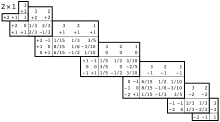
\includegraphics[width=0.8\textwidth]{coefficients-table}
\end{figure}
%
\begin{enumerate}
    \item $\boldsymbol{L=3}$
        \begin{itemize}
            \item 
                $
                \Ket{3,3} = \eo{2,2} \et{1,1}
                $
            \item 
                $
                \Ket{3,2} = \sqrt{\frac{1}{3}} \left( \eo{2,2} \et{1,0} + \sqrt{2} \eo{2,1} \et{1,1} \right)
                $
            \item 
                $ 
                \Ket{3,1} = 
                \sqrt{\frac{1}{30}} \left( \sqrt{2} \eo{2,2} \et{1,-1} + 4 \eo{2,1} \et{1,0} + 2\sqrt{3} \eo{2,0} \et{1,1} \right)
                $
            \item
                $ 
                \Ket{3,0} =
                \sqrt{\frac{1}{5}} \left( \eo{2,1} \et{1,-1} + \sqrt{3} \eo{2,0} \et{1,0} + \eo{2,-1} \et{1,1} \right)
                $
            \item 
                $
                \Ket{3,-1} =
                \sqrt{\frac{1}{15}} \left( \sqrt{6} \eo{2,0} \et{1,-1} + 2\sqrt{2} \eo{2,-1} \et{1,0} + \eo{2,-2} \et{1,1} \right)
                $
            \item
                $
                \Ket{3,-2} =
                \sqrt{\frac{1}{3}} \left( \sqrt{2} \eo{2,-1} \et{1,-1} + \eo{2,-2} \et{1,0} \right)
                $
            \item 
                $
                \Ket{3,-3} = \eo{2,-2} \et{1,-1}
                $
        \end{itemize}
        %
    \item $\boldsymbol{L=2}$
        \begin{itemize}
            \item 
                $
                \Ket{2,2} =
                \sqrt{\frac{1}{3}} \left( \sqrt{2} \eo{2,2} \et{1,0} - \eo{2,1} \et{1,1} \right)
                $
           \item 
                $
                \Ket{2,1} =
                \sqrt{\frac{1}{6}} \left( \sqrt{2} \eo{2,2} \et{1,-1} + \eo{2,1} \et{1,0} - \sqrt{3} \eo{2,0} \et{1,1} \right)
                $
            \item
                $
                \Ket{2,0} = \sqrt{\frac{1}{2}} \left( \eo{2,1} \et{1,-1} - \eo{2,-1} \et{1,1} \right)
                $
            \item
                $
                \Ket{2,-1} = 
                \sqrt{\frac{1}{6}} \left( - \sqrt{3} \eo{2,0} \et{1,-1} + \eo{2,-1} \et{1,0} + \sqrt{2} \eo{2,-2}  \et{1,1} \right)
                $
            \item
                $
                \Ket{2,-2} =
                \sqrt{\frac{1}{3}} \left( - \eo{2,-1} \et{1,-1} + \sqrt{2} \eo{2,-2} \et{1,0} \right)
                $
        \end{itemize}
    \item $\boldsymbol{L=1}$
        \begin{itemize}
           \item 
                $
                \Ket{1,1} =
                \sqrt{\frac{1}{10}} \left( \sqrt{6} \eo{2,2} \et{1,-1} -\sqrt{3} \eo{2,1} \et{1,0} + \eo{2,0} \et{1,1} \right)
                $
            \item
                $
                \Ket{1,0} = 
                \sqrt{\frac{1}{10}} \left( \sqrt{3} \eo{2,1} \et{1,-1} - 2 \eo{2,0} \et{1,0}  + \sqrt{3} \eo{2,-1} \et{1,1} \right)
                $
            \item
                $
                \Ket{1,-1} = 
                \sqrt{\frac{1}{10}} \left( \eo{2,0} \et{1,-1} - \sqrt{3} \eo{2,-1} \et{1,0} + \sqrt{6} \eo{2,-2} \et{1,1}  \right)
                $
        \end{itemize}
\end{enumerate}

%
% --- Bibliografía ---
%
% \clearpage
% \newpage
% \addcontentsline{toc}{section}{Bibliografía}
% \printbibliography[title={References}] % change from bibliography to references
% \printbibliography
% \nocite{*}
% \bibliographystyle{apalike}
% \bibliography{/home/jose/Documents/latex/preamble/references.bib}
% \clearpage
%%%%%%%%%%%%%%%%%%%%%%%%%%
\end{document}
